%%%%%%%%%%%%%%%%%%%%%%%%%%%%%%%%%%%%%%%%%
% Journal Article
% LaTeX Template
% Version 1.4 (15/5/16)
%
% This template has been downloaded from:
% http://www.LaTeXTemplates.com
%
% Original author:
% Frits Wenneker (http://www.howtotex.com) with extensive modifications by
% Vel (vel@LaTeXTemplates.com)
%
% License:
% CC BY-NC-SA 3.0 (http://creativecommons.org/licenses/by-nc-sa/3.0/)
%
%%%%%%%%%%%%%%%%%%%%%%%%%%%%%%%%%%%%%%%%%

%----------------------------------------------------------------------------------------
%	PACKAGES AND OTHER DOCUMENT CONFIGURATIONS
%----------------------------------------------------------------------------------------

\documentclass[10pt]{article} % Single column

%\documentclass[twoside,twocolumn]{article} % Two column

\usepackage{blindtext} % Package to generate dummy text throughout this template 

\usepackage[sc]{mathpazo} % Use the Palatino font
\usepackage[T1]{fontenc} % Use 8-bit encoding that has 256 glyphs
\linespread{1.05} % Line spacing - Palatino needs more space between lines
\usepackage{microtype} % Slightly tweak font spacing for aesthetics

\usepackage[spanish]{babel} % Language hyphenation and typographical rules

\usepackage[hmarginratio=1:1,top=32mm,columnsep=20pt]{geometry} % Document margins
\usepackage[hang, small,labelfont=bf,up,textfont=it,up]{caption} % Custom captions under/above floats in tables or figures
\usepackage{booktabs} % Horizontal rules in tables

\usepackage{lettrine} % The lettrine is the first enlarged letter at the beginning of the text

\usepackage{enumitem} % Customized lists
\setlist[itemize]{noitemsep} % Make itemize lists more compact

\usepackage{abstract} % Allows abstract customization
\renewcommand{\abstractnamefont}{\normalfont\bfseries} % Set the "Abstract" text to bold
\renewcommand{\abstracttextfont}{\normalfont\small\itshape} % Set the abstract itself to small italic text

\usepackage{titlesec} % Allows customization of titles
\renewcommand\thesection{\Roman{section}} % Roman numerals for the sections
\renewcommand\thesubsection{\roman{subsection}} % roman numerals for subsections
\titleformat{\section}[block]{\large\scshape\centering}{\thesection.}{1em}{} % Change the look of the section titles
\titleformat{\subsection}[block]{\large}{\thesubsection.}{1em}{} % Change the look of the section titles

\usepackage{fancyhdr} % Headers and footers
\pagestyle{fancy} % All pages have headers and footers
\fancyhead{} % Blank out the default header
\fancyfoot{} % Blank out the default footer
\fancyhead[C]{Sistemas Distribuidos. \textbf{Monica Scheduler}} % Custom header text
\fancyfoot[RO,LE]{\thepage} % Custom footer text

\usepackage{titling} % Customizing the title section

\usepackage{hyperref} % For hyperlinks in the PDF

\usepackage{graphicx} % For images

\usepackage{pifont} % bullets

\usepackage{amsmath}

\usepackage{algpseudocode}

\usepackage{float}
% Keywords command
\providecommand{\keywords}[1]
{
	\small	
	\vspace{0.5em}
	\noindent \textbf{\textit{Palabras clave --- }} #1
}


%----------------------------------------------------------------------------------------
%	TITLE SECTION
%----------------------------------------------------------------------------------------

\setlength{\droptitle}{-4\baselineskip} % Move the title up

\pretitle{\begin{center}\Huge\bfseries} % Article title formatting
	\posttitle{\end{center}} % Article title closing formatting
\title{\normalsize{Sistemas Distribuidos}\\
	\Huge\bfseries Monica Scheduler \\
} % Article title
\author{% 
	% \includegraphics[width=15em]{logo.png}\\
	Laura Victoria Riera P\'erez\\
	Mari\'e del Valle Reyes \vspace{1em} \\
	\small Cuarto a\~no. Ciencias de la Computaci\'on. \\ % institution
	\small Facultad de Matem\'atica y Computaci\'on, Universidad de La Habana, Cuba \\ % institution
}
\date{\footnotesize \today } % Leave empty to omit a date


% Abstract configurations
\renewenvironment{abstract}
{\small
	\begin{center}
		\bfseries \abstractname\vspace{-.5em}\vspace{0pt}
	\end{center}
	\list{}{
		\setlength{\leftmargin}{1.5cm}%
		\setlength{\rightmargin}{\leftmargin}%
	}%
	\item\relax}
{\endlist}

\usepackage{amsthm}
\usepackage{amssymb}
\usepackage{todonotes} % \TODO
\usepackage{listings} % Code listings
\usepackage{xcolor}

\definecolor{backcolour}{rgb}{0.95,0.95,0.92}

\newcommand{\csl}[1]{\colorbox{backcolour}{\texttt{#1}}}

\newcommand{\imgcaption}[2]{\tiny \textbf{Figura #1.} #2.}

\newcommand{\mgc}[2][]{\colorbox{backcolour}{\texttt{\_\_#2\_\_#1}}}

\newcommand{\mgccapt}[1]{\texttt{\_\_#1\_\_}}

\newtheorem{thm}{Teorema}
\newtheorem{mydef}{Definici\'on}%[section]
\newtheorem{lem}{Lema}
\newtheorem{fig}{\scriptsize{Figura}}


\renewcommand{\qedsymbol}{\rule{0.7em}{0.7em}}

% Hyperlinks configurations
\hypersetup{
	colorlinks=true,
	linkcolor=black,
	filecolor=magenta,      
	urlcolor=cyan,
	pdftitle={Overleaf Example},
	pdfpagemode=FullScreen,
}

%----------------------------------------------------------------------------------------

\begin{document}
	
	\bibliographystyle{ieeetr}
	
	% Print the title
	\maketitle
	
	%----------------------------------------------------------------------------------------
	%	ARTICLE CONTENTS
	%----------------------------------------------------------------------------------------
	
	\section*{Repositorio del proyecto}
	
	\begin{center}
		\href{https://github.com/computer-science-crows/monica-scheduler}{https://github.com/computer-science-crows/monica-scheduler}
	\end{center}

	\section{Definici\'on inicial del problema} 
	
	El tiempo es un recurso de vital importancia. Una de las estrategias más comunes para su gestión es el uso de una agenda, para la cual existen diversas opciones que abarcan desde el formato tradicional en papel hasta las versiones electrónicas modernas. Sin embargo, debido a la naturaleza intrínseca de las interacciones humanas, una agenda personal a menudo resulta insuficiente. En numerosas ocasiones, es imprescindible coordinarla con otras personas para llevar a cabo actividades conjuntas. Este proceso implica la identificación de horarios compartidos y la detección de intervalos de tiempo libres. Además, estas planificaciones pueden verse alteradas por eventos imprevistos a los que se debe asistir, lo que conlleva la necesidad de modificar la agenda nuevamente.
	
	Este proyecto consiste en crear una agenda distribuida como herramienta de gest\'ion del tiempo para eventos personales o grupales. Los requisitos clave para este sistema son:
	\begin{enumerate}
		\item \textbf{Arquitectura Distribuida}: El sistema debe ser diseñado e implementado como un sistema distribuido. Esto significa que el sistema debe ser capaz de funcionar en múltiples máquinas mientras se presenta a los usuarios como un sistema coherente único.
		
		\item \textbf{Mecanismo de Autenticación e Identificación}: El sistema debe ser capaz de autenticar e identificar a cada usuario. Esto asegura que solo los usuarios autorizados puedan acceder al sistema y realizar ciertas acciones.
		
		\item \textbf{Formación Dinámica de Grupos}: El sistema debe permitir la creación dinámica de grupos, ya sean jerárquicos o no jerárquicos. Esto significa que los usuarios deben poder crear y gestionar grupos dentro del sistema de manera flexible.
		
		\item \textbf{Citas Grupales}: El sistema debe admitir la creación de citas grupales. Si se utiliza un grupo jerárquico, una cita creada por un superior debe aparecer automáticamente en las agendas de todos los miembros del grupo. Para grupos no jerárquicos, todos los miembros deben aceptar la cita para que se confirme.
		
		\item \textbf{Actualizaciones Automáticas de la Agenda}: Cuando se crea, modifica o elimina una cita, los cambios deben reflejarse automáticamente en las agendas de los usuarios relevantes.
		
		\item \textbf{Identificación de Conflictos}: El sistema debe ser capaz de identificar conflictos en las agendas locales. Por ejemplo, si un usuario tiene programadas dos citas al mismo tiempo, el sistema debe señalar esto como un conflicto.
		
		\item \textbf{Visualización de la Agenda}: Los usuarios deben poder ver las agendas de un grupo de personas durante un período de tiempo determinado. El sistema debe respetar la privacidad de la información del usuario y los niveles jerárquicos al mostrar esta información.
	\end{enumerate}
	
	\section{Modelaci\'on del problema}
	
	\begin{figure}[H]
		\centering
		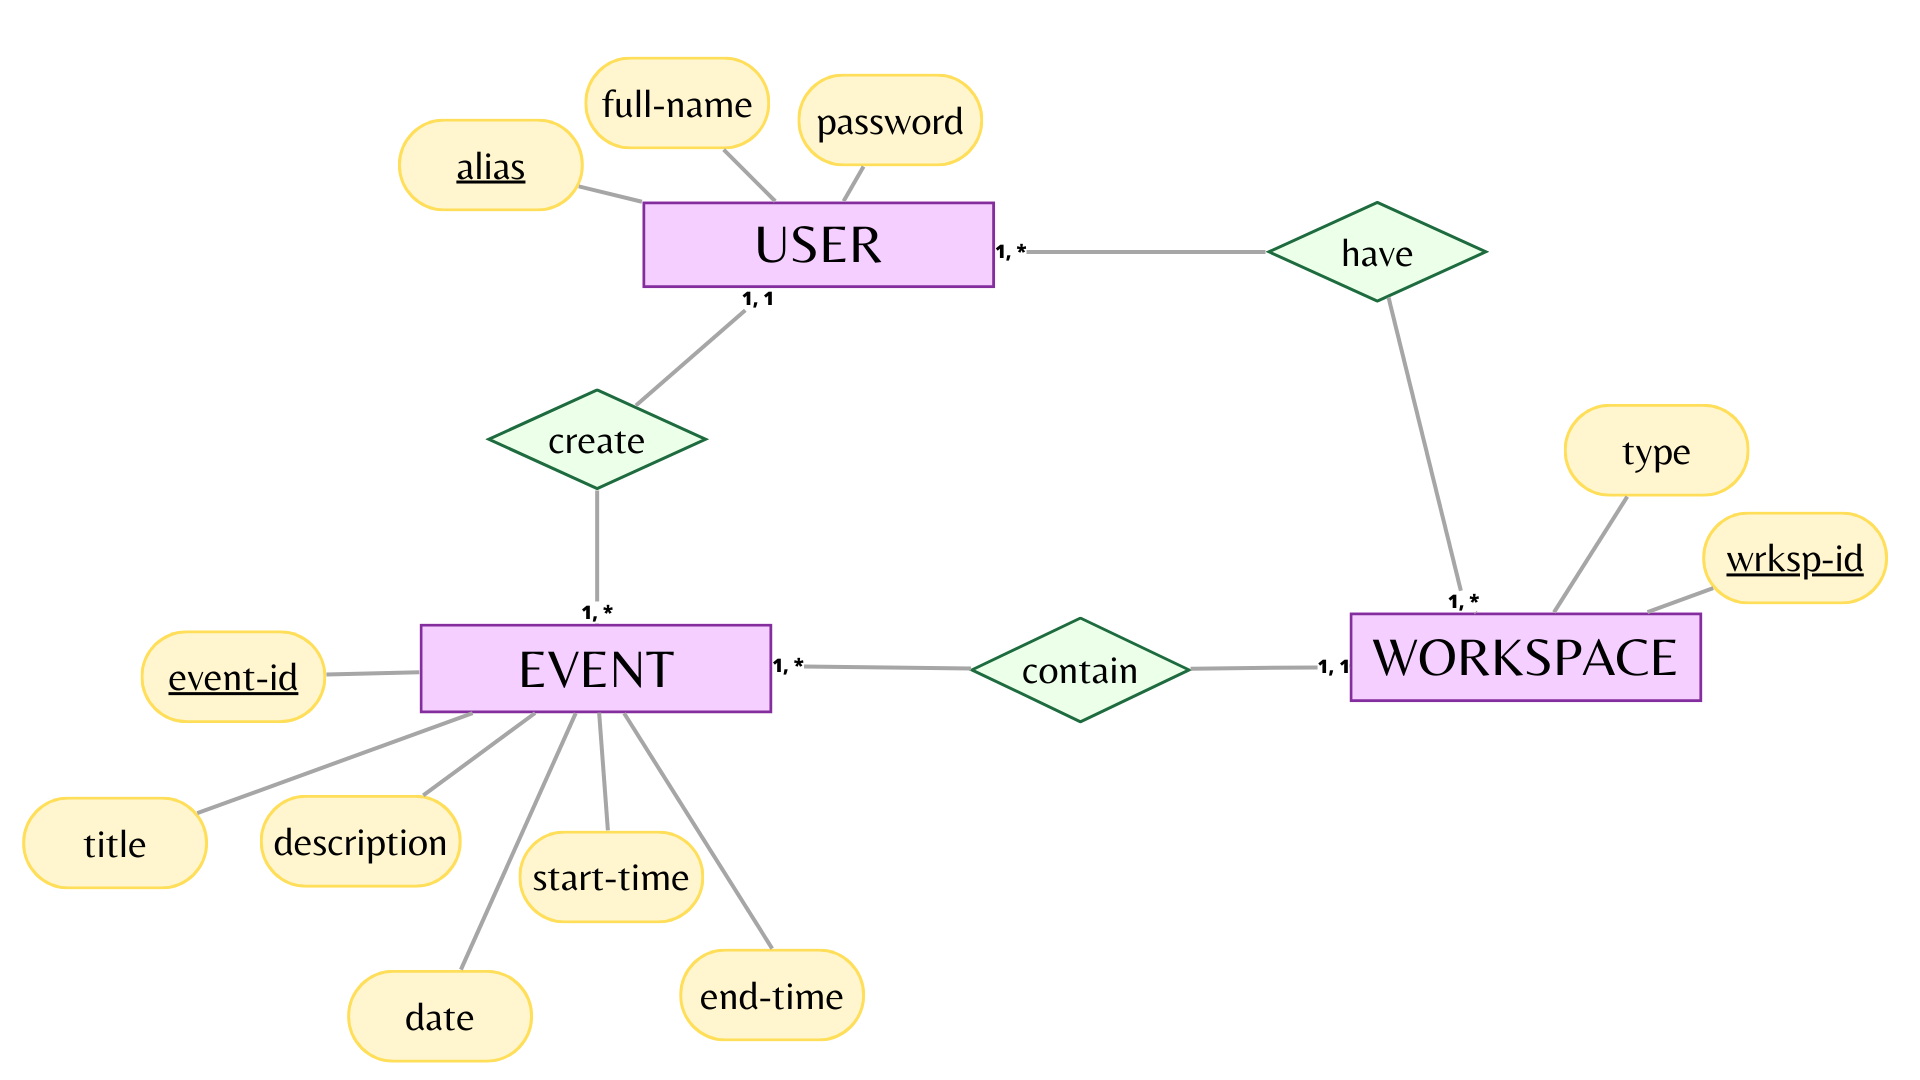
\includegraphics[width=10cm]{merx.png}
		\caption{text}
	\end{figure}
	
	\section{Herramientas utilizadas}
	
	\begin{itemize}
		\item docker
		\item MongoDB
		\item FastAPI
		\item React
	\end{itemize}
	
	\section{Arquitectura: Microservicios}
	
	Microservices architecture, also known simply as microservices, is an architectural style that structures an application as a collection of small autonomous services, modeled around a business domain.
	
	Services definition:
	Technology stack:
	
	\section{DHT}
	
	Una DHT (Tabla Hash Distribuida) es una estructura de datos que se utiliza en sistemas distribuidos para almacenar pares de clave-valor de manera eficiente.
	
	Propiedades:
	
	\begin{itemize}
		\item  Distribución: Los datos se distribuyen entre todos los nodos de la red, lo que significa que no hay un único punto de fallo y que la red puede escalar a un gran número de nodos.
		
		\item  Descentralización: No hay un nodo central o coordinador en una DHT. Cada nodo puede funcionar de manera independiente y sólo necesita saber sobre un pequeño número de otros nodos.
		
		\item  Eficiencia: Las DHT pueden realizar operaciones de búsqueda, inserción y eliminación de datos en un tiempo logarítmico con respecto al número de nodos en la red.
		
		\item Resistencia a fallos: Las DHT suelen ser resistentes a fallos, lo que significa que pueden seguir funcionando incluso cuando algunos nodos de la red fallan o se desconectan.
	\end{itemize}
	
	\subsection{Kademlia}
	
	La implementación de una Tabla Hash Distribuida (DHT) de Kademlia implica varios componentes clave. 
	
	Descripción general de elementos a implementar:
	
	\subsubsection{Nodo}
	
	\subsubsection{IDs de Nodo}
	
	Cada nodo en la red debe tener un identificador único. En Kademlia, este suele ser un número de 160 bits, a menudo generado usando una función hash como SHA-1.
	
	\subsubsection{Almacenamiento de Clave-Valor} 
	
	Cada nodo debe mantener un almacenamiento local de clave-valor. Estos son los datos de los que el nodo es responsable en la DHT.
	
	\subsubsection{Tabla de Enrutamiento}
	
	 Cada nodo debe mantener una lista de otros nodos en la red, ordenados por la distancia entre sus IDs de nodo y el suyo propio. Kademlia utiliza una estructura de datos específica llamada k-bucket para hacer esto.
	
	\subsubsection{Operaciones de Red} 
	
	Necesitarás implementar varias operaciones que los nodos pueden realizar a través de la red:
	
	\begin{itemize}
		\item  `PING`: Verificar si otro nodo está en línea.
		\item  `STORE`: Almacenar un par clave-valor en un nodo.
		\item  `FIND\_NODE`: Encontrar los k nodos más cercanos a una clave dada.
		\item  `FIND\_VALUE`: Recuperar un valor por su clave si el nodo lo tiene, o los k nodos más cercanos a la clave en caso contrario.
	\end{itemize}
	
	\subsubsection{Proceso de Ingreso de Nodo} 
	
	Cuando un nuevo nodo se une a la red, necesita poblar su tabla de enrutamiento. Hace esto realizando una operación `FIND\_NODE` en su propia ID.
	
	\subsubsection{Replicación y Republicación de Valores} 
	
	Para asegurar que los datos no se pierdan cuando los nodos abandonan la red, Kademlia almacena múltiples copias de cada par clave-valor en diferentes nodos. Necesitarás implementar esta replicación, así como un proceso para que los nodos republiquen periódicamente sus pares clave-valor.
	
	\subsubsection{Manejo de Fallos de Nodo} 
	
	Los nodos necesitan verificar periódicamente si sus pares aún están en línea y actualizar sus tablas de enrutamiento en consecuencia.
	
	\subsubsection{Concurrencia} 
	
	Kademlia utiliza muchas operaciones concurrentes para acelerar las operaciones de red y hacer la red más robusta. Tendrás que manejar esto en tu implementación.
	
	\subsubsection{Comunicaci\'on: RPCs}
	
	\subsubsection{Consistencia y Replicaci\'on: Active replication}
	
	Active replication, also known as state machine replication, is a strategy where each operation is performed on all replicas. This ensures that all replicas have the same state at any given time. Here's a basic outline of how it could work in your distributed agenda system:
	
	1. **Operation Invocation**: When a client wants to perform an operation (like creating a new event in the agenda), it sends a request to a designated component in your system. This could be a load balancer, a leader node in a consensus protocol, or any other component that's responsible for coordinating requests.
	
	2. **Broadcast to Replicas**: The coordinating component then broadcasts the operation to all replicas. This could be done through a variety of methods, such as multicast or a publish-subscribe system. The important part is that all replicas receive the operation.
	
	3. **Perform Operation**: Each replica independently performs the operation. Since all replicas are identical and receive the same sequence of operations, they should all arrive at the same state. For example, if the operation was to create a new event, each replica would add that event to its copy of the agenda.
	
	4. **Response to Client**: After performing the operation, each replica sends a response back to the coordinating component. Once the coordinator has received responses from all replicas (or a sufficient number of them), it sends a final response back to the client.
	
	5. **Error Handling**: If any replica fails to perform the operation, the system needs to handle this error. This could involve retrying the operation, removing the faulty replica, or other error recovery strategies.
	
	Remember, the key to active replication is ensuring that all replicas perform every operation in the same order. This often requires careful coordination and can introduce significant complexity into your system. But when done correctly, it can provide a high degree of reliability and fault tolerance.
	
	\subsubsection{Tolerancia a Fallas}
	
	\section{Seguridad}
	
	Security in distributed systems is concerned with the prevention and detection of unauthorized actions by users of a system. The security of a distributed system can be divided into two main parts: secure channels and secure processes. Secure channels are used to protect data from being intercepted or tampered with during transmission. Secure processes are used to ensure that only authorized users can access and manipulate data.
		
	\subsection{Autenticaci\'on}
	
	\subsection{Autorizaci\'on}
	
	\bibliography{refs} 
\end{document}


